\documentclass{presentation}

\title{MQTT}
\subtitle{IoT for Wisconsin Chemists}
\author{Blaise Thompson}

\institute{University of Wisconsin--Madison}
\date{\today}

\begin{document}
\maketitle

\section{MQTT}

\begin{frame}{MQTT}
  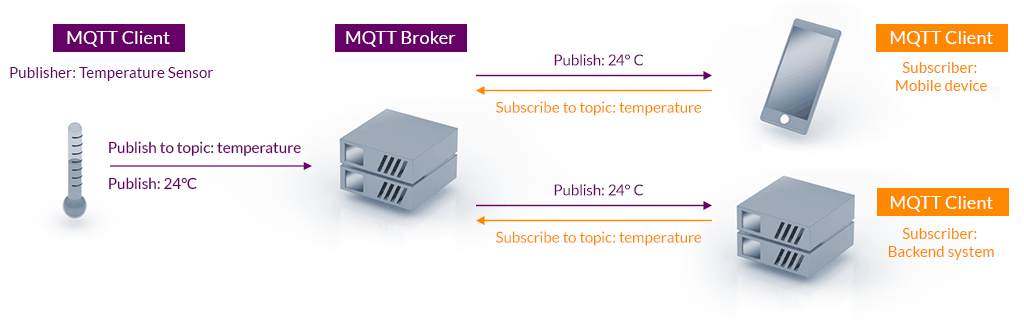
\includegraphics[width=\textwidth]{./mqtt-publish-subscribe.png}
  Graphic from https://mqtt.org/
\end{frame}

\begin{frame}{mosquitto}
  
\includegraphics[width=\textwidth/4]{./mosquitto-text-side-28.png} \\
  https://mosquitto.org/download/ \\
  \vfill
  \texttt{mosquitto\_sub -h mqtt.chem.wisc.edu -t "\#" -{}-verbose} \\
  \vfill
  \texttt{-t "homie/+/+/temperature"}
  \vfill
  \texttt{mosquitto\_pub ...}
  \vfill
\end{frame}

\begin{frame}{Python}
	\texttt{pip install paho-mqtt}
	\vfill
	\texttt{conda install paho-mqtt}
\end{frame}

\begin{frame}{Python}
	\url{https://gist.github.com/untzag/32ce545cdf315419af6174c71562b7c4}
\end{frame}

\begin{frame}{QoS}
  Quality of Sevice level
  \begin{itemize}
    \item{0 - at most once}
    \item{1 - at least once}
    \item{2 - exactly once}
  \end{itemize}
  More quality is more expensive on the network.
\end{frame}

\begin{frame}{Retention}
  Retention
\end{frame}

\section{Homie}

\begin{frame}{Homie}
  \center
  
\includegraphics[width=\textwidth/3]{./Homie-logo.png} \\
  https://homieiot.github.io/
\end{frame}

\begin{frame}{Homie}
  \vfill
  {\huge homie/device/node/property}
  \vfill
  A convention for structured MQTT data.
\end{frame}

\begin{frame}{Homie}
  \vfill
  {\huge homie/device/node/property}
  \texttt{
  \vfill
  homie/device123/\$homie → 4.0.0 \\
  homie/device123/\$name → My device \\
  homie/device123/\$state → ready \\ 
  homie/device123/\$nodes → mythermostat \\
  }
\end{frame}


\begin{frame}{Homie}
  \vfill
  {\huge homie/device/node/property}
  \texttt{
  \vfill
  .../device123/mythermostat/\$name → My thermostat  \\
  .../device123/mythermostat/\$properties → temperature \\
  }
\end{frame}

\begin{frame}{Homie}
  \vfill
  {\huge homie/device/node/property}
  \texttt{
  \vfill
  .../mythermostat/temperature → 22 \\
  .../mythermostat/temperature/\$name → Temperature \\
  .../mythermostat/temperature/\$unit → deg\_C \\
  .../mythermostat/temperature/\$datatype → integer \\
  .../mythermostat/temperature/\$settable → false \\
  }
\end{frame}

\begin{frame}{Homie}
  \begin{columns}
    \begin{column}{0.5\textwidth}
      Property datatype options
      \begin{itemize}
        \item string
        \item integer
        \item float
        \item percent
        \item boolean
        \item enum
        \item color (rgb, hsv)
        \item datetime (ISO 8601)
        \item duration (ISO 8601)
      \end{itemize}
    \end{column}
    \begin{column}{0.5\textwidth}
      Units
      \begin{itemize}
        \item anything you want
	\item reccomend standard unit strings
        \item pint library
      \end{itemize}
    \end{column}
  \end{columns}
\end{frame}

\begin{frame}{Homie}
  Feed data how you wish...
  \begin{itemize}
    \item{manually with generic MQTT client}
    \item{microhomie, ESP8266}
    \item{https://github.com/mjcumming/Homie4}
  \end{itemize}
\end{frame}

\section{Graphite}

\begin{frame}{Graphite}
  \center
  
\includegraphics[width=\textwidth/2]{./Graphite.png} \\
  https://graphiteapp.org \\
  http://graphite.chem.wisc.edu
\end{frame}

\begin{frame}{Graphite}
  \begin{columns}
    \begin{column}{0.5\textwidth}
      all published topics which...
      \begin{itemize}
        \item follow Homie convention
        \item is numerical
      \end{itemize}
      ...gets stored to Graphite
    \end{column}
    \begin{column}{0.5\textwidth}
      Data aggregated
      \begin{itemize}
        \item 12 seconds for 10 days
        \item 2 minutes for 100 days
	\item 2 hours for 10 years
      \end{itemize}
      Downsampled via averaging
    \end{column}
  \end{columns}
\end{frame}

\begin{frame}{Graphite}
  render
  \vfill
  http://graphite.chem.wisc.edu/render/ \\
	?width=704 \\
	\&height=500 \\
	\&fontSize=18 \\
	\&target=shop.weather.000000.bme680.temperature \\
	\&from=-1w \\
  \vfill
  \&format=csv  
\end{frame}

\begin{frame}{Graphite}
  render
  \vfill
  http://graphite.chem.wisc.edu/render/ \\
	?width=704 \\
	\&height=500 \\
	\&fontSize=18 \\
	\&target=shop.weather.000000.bme680.temperature \\
	\&target=shop.weather.000001.bme680.temperature \\
	\&from=-1w \\
  \vfill
  \&format=csv  
\end{frame}

\begin{frame}{Graphite}
  render
  \vfill
  http://graphite.chem.wisc.edu/render/ \\
	?width=704 \\
	\&height=500 \\
	\&fontSize=18 \\
	\&target=aliasByNode(room.weather.*.*.*.temperature,2) \\
	\&from=-1w \\
  \vfill
  \&format=csv  
\end{frame}

\begin{frame}{Graphite}
  dashboard websites
\end{frame}

\begin{frame}{Warnings}
  \begin{itemize}
    \item Broker WILL go down occasionally
    \item Database WILL go down occasionally
    \item  Data is NOT permanent
    \item Things WILL change
    \item Do not use for crucial control
  \end{itemize}
\end{frame}




\end{document}
